% vim: set tw=78 sts=2 sw=2 ts=8 aw et ai:
\documentclass[conference]{IEEEtran}

\usepackage{ucs}
\usepackage{url}
\usepackage[utf8x]{inputenc}
\usepackage[english]{babel}
%\usepackage{hyperref}	  % use \url{http://$URL} or \href{http://$URL}{Name}
\usepackage{underscore}	  % underscores need not be escaped
\usepackage{subfigure}
\usepackage{verbatim}
\usepackage{float}
\usepackage{amsmath, amsthm, amssymb}
\usepackage{parskip}
\usepackage{flushend}

% Support for including graphics
\usepackage{graphicx}
\DeclareGraphicsExtensions{.pdf,.png,.jpg}

\begin{document}


\title{Geodynamics monitorization using wireless sensor networks}

\author{
\IEEEauthorblockN{Andrei-Alexandru Mușat}
\IEEEauthorblockA{
  Automatic Control and Computers Faculty\\
  University Politehnica of Bucharest,\\
  \{andrei.musat@cti.pub.ro\}}
  }


 
\maketitle

\begin{abstract} 
Wireless sensor networks are a cheap and versatile solution for monitoring various environments 
and elements of an environment. There exists a number of such applications used worldwide to monitor 
areas in which human access is hard or near impossible. The issue with these applications is that 
they are mainly used by government organizations or for research purposes. They seldom focus on 
using the data in the interest of safety for the population, such as warning them of natural 
disasters or assessing the risk of damaged areas left in the wake of a natural disaster. The 
solution we propose in this article is a low power, low cost wireless sensor which is used to 
monitor earthquakes and the status of urban structures exposed to earthquakes or other sources 
of vibration in order to prevent possible disasters.

\end{abstract}

\begin{IEEEkeywords}
Wireless Sensor Networks, Geodynamics, Earthquake monitoring, Low power
\end{IEEEkeywords}

\section{Introduction}
\label{sec:introduction}
Wireless Sensor Networks are being used more and more in almost every field imaginable in order to collect and improve our life, fileds like home automation, agriculture, military, space exploration etc. In order to collect the data, gateway platforms \cite{hill2004platforms,da2011design,da2011design2} are required and most of them are stationary bulky devices or PCs connected to one of the wireless nodes that serve as a base-station. We aim to show in this paper that there exists a solution for a truly mobile gateway design that can be used either for collecting data or for debuging large wireless network infrastructures.

We have conected to an AR Parrot Drone 2.0 our SparrowDongle, a USB stick featuring two microcontrollers that can connect to 2.4GHz Zigbee nodes or to our own node design Sparrowv3.2. We will show an overview of the system
architecture in Chapter \ref{chap:arch}, the hardware and software
implementation in Chapter \ref{chap:impl} and results of using the gateway in
Chapter \ref{chap:results}. 

\begin{figure}[ht] \centering
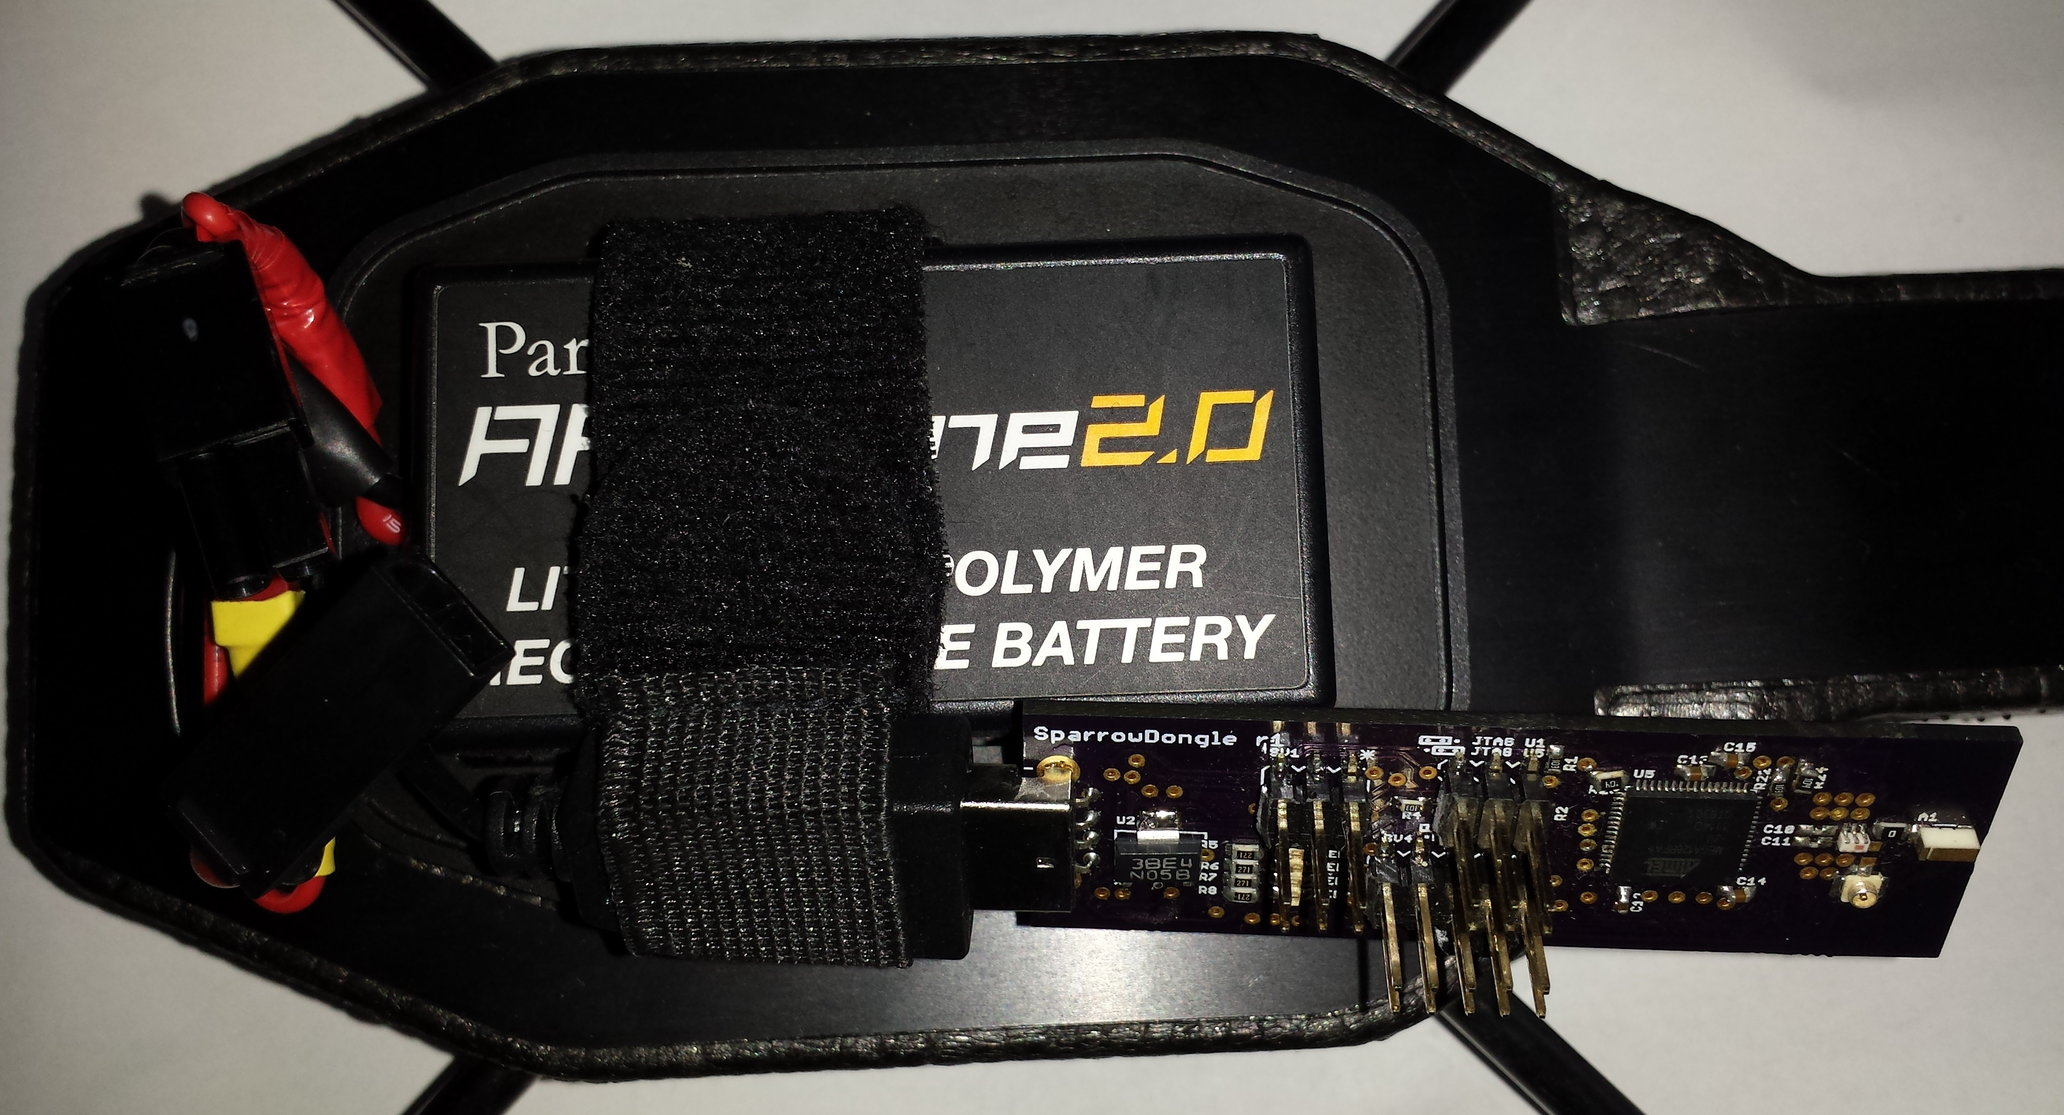
\includegraphics[width=0.45\textwidth]{img/dronedongle.jpg} \caption{SparrowDongle connected to AR Parrot Drone 2.0 } \end{figure}




\section{Related Work}
\label{sec:related}
\normalfont\normalsize
\chapter{Related Work}

The related work is starting the expand and new researches propose new ideas, but generaly speaking they tend to focus on ways of collecting the data from the nodes. The objective in their articles is to see if an UAV can be integreated with a wireless sensor networks. The conclusion is generaly positive, but a big problem in adopting their research in real life scenarios is represented by the high costs of the equipment they used and the necesary knowledge required to setup and operate the equipment.

The general experiments presented in the UAV and WSN integeration research are the following:

\begin{itemize}

\item Usign nodes signal to perform course corections for dynamic navigation
\item Data muling from nodes 
\item Using drones to deploy a new node in order to expand or to fix a problem in the network
\item Using drones to determine ground military activity \cite{akyildiz2002wireless}

\end{itemize}


\section{Standard WSN Protocols}

The protocols implemented in Wireless Sensor Network are based on sourounding node discovery in order to build a topology and find the best way they can multihop data to the gateway. This approach works best in a static environment, but in a dynamic environment or an eviroment were the distance between nodes is too big or the time between two data packets is too big, the network convergence will be slow or not even possible.

\section{UAV experiments with Wireless Sensor Networks} \cite{teh2008experiments} 

The experiment consisted of using ground nodes that had a gps position assigned. The UAV plane would performe course corection after receiving the curent gps position from the node in order to calculate the best path for muling the data from the nodes.

The advantage of using a plane used for the experiment is the longer range and higher speed that it can offer against a quadcopter or a similiar design.  But the high speed creates the problem of maneuverability. The plane has a turning range of 400 meters while the drone can almost turn on the same spot.

\section{Crop Monitoring} \cite{valente2011air}

A research of using a drone for crop monitoring has been conducted at a vineyard. Their system was comprised of a unmanned quadcopter, an Arduino board with a GPRS module for long distance communication with  the drone and ZigBee and Crossbow’s TelosB as wireless sensing nodes. The drone was not controlled via the long-distance link, but through a Spektrum DX7SE 2.4 GHz remote control.

They demonstrated that a preprogramed UAV can be used to monitor multiple crops where a standard WSN could not be deployed because of the unique constrains imposed by the environment.

The cost of the implementation was relatively high compared to ours, the remote is 300\$, the same as the entire drone that we propose and the TelosB is 99\$. This data suggests that for their experiment the drone, communication module and the remote control were half the cost of the equipment.

Another problem was that they were not saving the data localy, but sending it back to the base station where it was proccesed and saved. This can represent a problem because the system cannot function propely unless a base station is supplied.

\section{Aware platform}\cite{ollero2007aware}

The Aware platform, proposed by Ays. Egül Tüysüz Erman, Lodewijk Van Hoesel and Paul Havinga from University of Twente, is a platform that integrates WSNs, UAVs, and actuators into a disaster response setting and provides facilities for event detection, autonomous network repair by UAVs, and quick response by integrated operational forces.

They use multiple UAVs to deploy new nodes that will replace the damaged ones and check if they function. The entire system still relies on a sink to collect the data and to send them to a base station.\cite{erman2008enabling}



\bibliographystyle{abbrv}
\bibliography{quake}

\end{document}
